\section{Regression}
As it is the most clinically relevant parameter,
and also the most demanding to measure,
we have chosen to attempt to predict the 2-hour serum insulin concentrations
from other, more easily determined variables
(excluding, of course, the class variable).
As we found in the previous report,
this attribute is of great importance to the dataset,
which is further reason to attempt to predict it.

\subsection{Linear regression}
We have used a linear regression with feature selection to predict the attribute.
A linear regression without feature selection 

\subsection{Artificial Neural Network}
An ANN with a large number of hidden units in several layers was constructed
(200 units in the first hidden layer, 100 in the second),
and standardization layers were placed before every layer but the last.
This maintains activations at a magnitude that assists in training the network.
As an additional consequence of placing a standardization before the first hidden layer,
the input data would also be normalized.

The loss function for the network was chosen to be the mean squared error.

The network was trained with 30\% of its data set held out as validation data,
and early stopping was employed, with training ending soon after the validation error
ceased to decrease.
This is cross-validation by holdout,
where the parameter is training time.
To see this,
imagine training a neural network for a wide range of training steps,
and then selecting the network that gives the lowest error
on some held-out validation data.
This is what we are doing,
except reusing the work done by previous training iterations
instead of training one network for 100 iterations,
then a different one for 101, etc.,
which would be a waste of computational power
and, due to random initialization of the weights at the beginning of training,
introduce large amounts of variance to the cross-validation process.

The early stopping procedure protects against overfitting,
and thus allows a more complex architecture to be used.
For this reason we have deliberately chosen a large number of hidden units
and, due to the large variance of training as well as the computational expense,
no cross-validation was performed to select between different numbers of hidden units
or other architectural features.

\subsection{Model comparison}


\section{Classification}

This data set contains an obvious binary attribute
with clinical relevance:
does the patient have diabetes or not?
As such, this question is what we will be
focusing our classification efforts on.

\subsection{Decision tree}
Decision trees are a way to split your training data into subsets. These splits are based on that attribute's value.
These subsets can then predict the datapoints' class. Decisions trees with the capacity to classify observations are called
classification trees. These trees sort the data by using Hunt's algorithm, which
splits the tree iteratively, and for each iteration keeps the split with the
highest purity gain. For this decisions tree, the "gini" impurity gain has been
chosen to quantify impurity gain. The algorithm can be stopped, and has indeed
been done so here, both by providing a maximum "depth" (or number of iterations
of splits) or by providing a minimum number of number of samples at a given
place in the tree to keep trying to improve the impurity.
The inner loop of a doubble-layered cross-validation for the decision tree
(which consisted of a leave-one-out cross-validation) showed
that the model is quite robust with regard to the tree-depth, which performed
best at the value of 3, given the following tree (when taken on all the available
data):

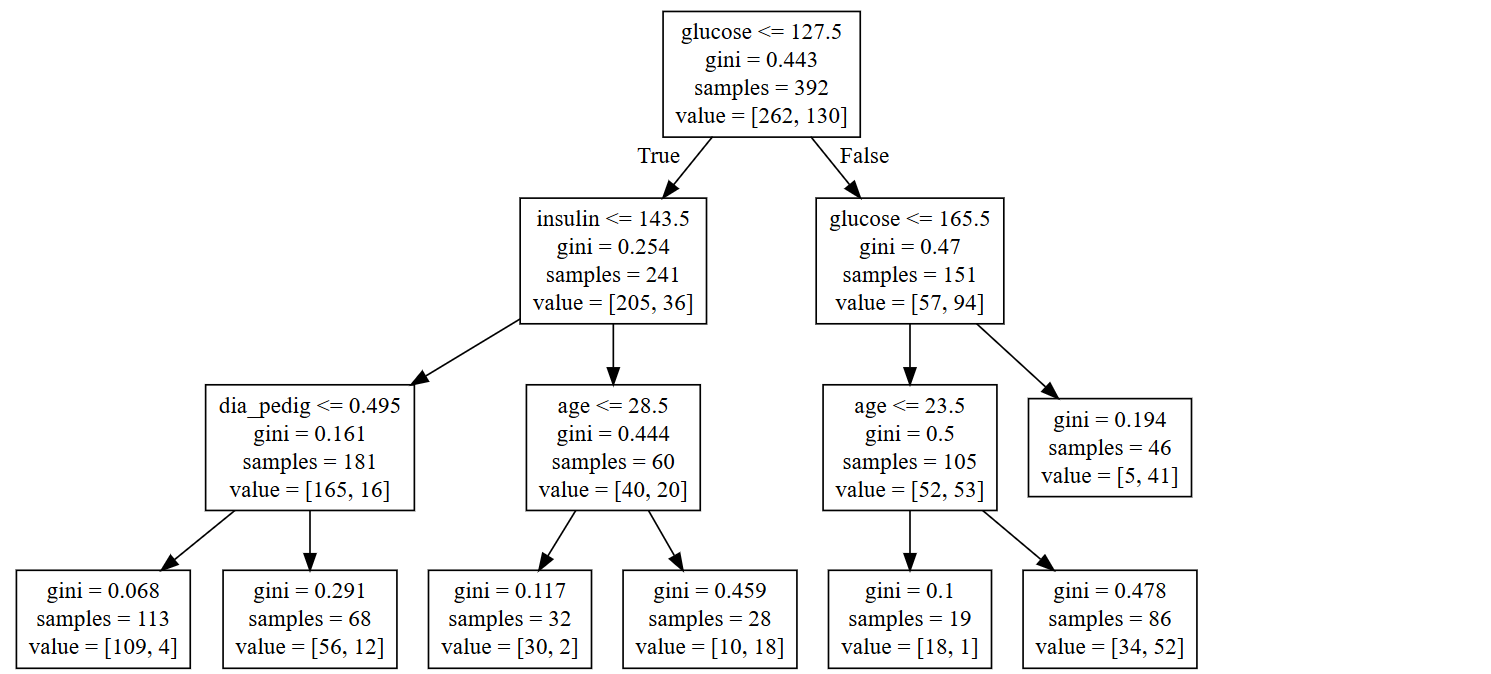
\includegraphics[width=\textwidth]{tree.png}

So, when given a datapoint, the first thing to do when using the tree to figure
out whether to classify a patient as with or without diabetes, is to ask whether
the patient's glucose level is equal to or below 127.5. If true, the insulin level
accounts for the next split, and if false, glucose once more, but with another
value this time, accounts for the split. Which box an observation or patient belongs
to in the last tier determines whether or not we believe the patient to have diabetes
or not.

\subsection{$k$-nearest neighbours}
The KNN-method takes a datapoints' K-amount of nearest neighbours and learns to predict the datapoints' class.
This is done by using the leave-one-out method and letting the model test the it's own ability to predict the classes.
The method is then repeated with a higher amount of neighbours and the test-error is then found. In our model, the nearest
neighbour will be the neighbour with the shortest euclidean distance to the observation.
This may become troublesome in higher-dimensional data, but with our 8 attributes, it should
not be too bad. The best number of neighbours were found in the inner loop with
the leave-one-out method, however, the best k's seem to change quite a bit for the
different data feeded to this loop by the outer loop, as can be seen below in the performance
tables. The best performing k can be seen to be 19, however, another k was
28 in the same run! This means that the parameter k for the model is not very
robust and is prone to change a lot. When the k has been chosen, the model then
predicts an observation's class based on its k nearest neighbours (as the
name suggests). This means that if the best performing k is 19, and the 10
data points that are closest to it by the euclidean distance is a given class,
then this class is chosen as the predicted class. This is hard to visualize
graphically because the dimension of our data is more than 3. Overall, this
method seems to perform similarly to the tree model.

\subsection{Artificial Neural Network}
The Artificial Neural Network learns a possibly non-linear function
over the dataset as a sequence of layers that each apply
a preferably non-linear function to an affine transformation of the vector arriving
``from below'' the layer.

There are various ways of training them with various risks of e.g.
getting stuck in local minima, but those are out of the scope of this report.

A network with the same structure as in the regression task was constructed and trained in the same way,
including early stopping.

The output layer was made to consist of two neurons,
with the activation function being softmax,
and the loss function was chosen to be Kullback–Leibler divergence
for its attractive interpretation as the relative entropy
of the output of the network with respect to the ground truth
represented by the training data.

\subsection{Model comparison}
We compared the ANN and the decision tree. We did this through finding their difference in accuracy rate.
The classifiers are seen as different if their accuracy rate is significantly different from zero. The better one being
the classifier being better at predicting correctly.
The "dummy"-predictor, predicting everyone to be healthy (or a zero) is also taken
into account and the results can be graphically seen below in Table 1 of accuracy rates:
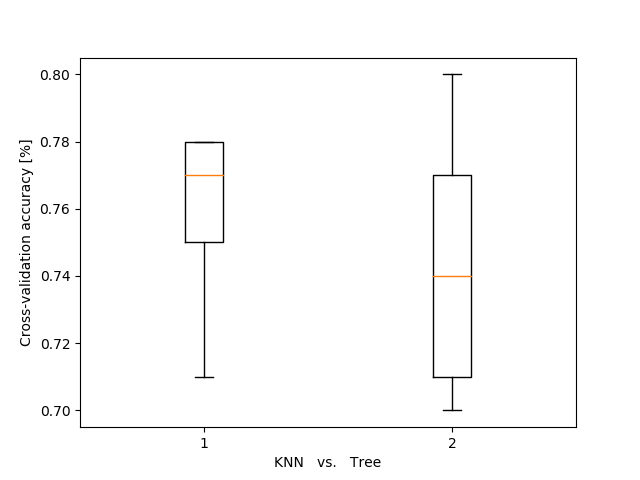
\includegraphics[width=\textwidth]{comp_knn_trees.png}
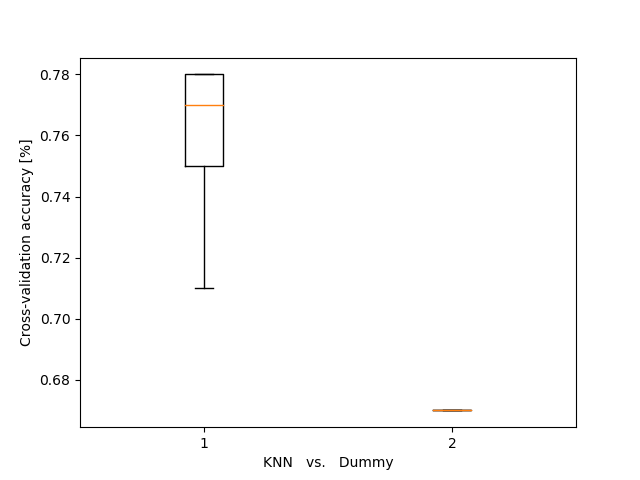
\includegraphics[width=\textwidth]{comp_knn_dummy.png}

The tests show that we cannot statistically differentiate between our two best models,
but they are statistically better than the dummy, which means the models beat just guessing
that the patients are just healthy.
The p-values were 0.55 for the best models and 0.0002 for the KNN and dummy comparison.
The dummy values have a low standard deviation, partly because we chose to use the
Stratified K-folds.

\begin{table}[Accuracy rates for the models]
\centering
\caption{Accuracy rates}
\label{my-label}
\begin{tabular}{@{}lllll@{}}
\toprule
fold                                                                      & KNN  & ANN  & Trees & Dummy &  \\ \midrule
\multicolumn{1}{|l|}{\cellcolor[HTML]{34FF34}{\color[HTML]{000000} 1}}    & 0.78 & 0.72 & 0.80  &  0.67 &  \\ \cmidrule(r){1-1}
\multicolumn{1}{|l|}{\cellcolor[HTML]{34FF34}{\color[HTML]{000000} 2}}    & 0.75 & 0.7 & 0.70  &  0.67 &  \\ \cmidrule(r){1-1}
\multicolumn{1}{|l|}{\cellcolor[HTML]{34FF34}{\color[HTML]{000000} 3}}    & 0.71 & 0.71 & 0.71  &  0.67 &  \\ \cmidrule(r){1-1}
\multicolumn{1}{|l|}{\cellcolor[HTML]{34FF34}{\color[HTML]{000000} 4}}    & 0.78 & 0.79 & 0.74  &  0.67 &  \\ \cmidrule(r){1-1}
\multicolumn{1}{|l|}{\cellcolor[HTML]{34FF34}{\color[HTML]{000000} 5}}    & 0.77 & 8.1 & 0.77  &  0.67  &  \\ \cmidrule(r){1-1}
\multicolumn{1}{|l|}{\cellcolor[HTML]{FFFFFF}{\color[HTML]{000000} mean}} & 0.76 & 7.4 & 0.74  &  0.67  &  \\ \cmidrule(r){1-1}
\multicolumn{1}{|l|}{\cellcolor[HTML]{FFFFFF}{\color[HTML]{000000} std}}  & 0.03 & 0.04 & 0.04  &  0.002  &  \\ \bottomrule
\end{tabular}
\end{table}

\section{Previous work}
There has been made previous work on the dataset.
An ANN was applied and there was developed an ADAP algorithm
which was used to forecast if the Pima Indians would develop diabetes within a 5 year period.
This algorithm was developed by the two authors [Smith, Dickson] in 1961.
The algorithm was trained using 576 cases, and thereafter tested on 192 cases. The model performed
with a precision of 76 per cent.




\appendix
\section{Distribution of responsibilities}
